\documentclass[conference]{IEEEtran}
\IEEEoverridecommandlockouts

\usepackage{cite}
\usepackage{amsmath,amssymb,amsfonts}
\usepackage{graphicx}
\graphicspath{{./}{figures/}}
\usepackage{textcomp}
\usepackage{xcolor}
\usepackage{booktabs}
\usepackage{subcaption}
\usepackage{url}

\makeatletter
\newcommand{\linebreakand}{%
  \end{@IEEEauthorhalign}
  \hfill\mbox{}\par
  \mbox{}\hfill\begin{@IEEEauthorhalign}
}
\makeatother

\begin{document}

\title{\textbf{High-Performance Parallelization of Pigeonhole\\Sort across\\MultiCore CPU Distributed MPI Clusters and\\NVIDIA CUDA GPUs}}

\author{
\IEEEauthorblockN{Bakkesh Y M R}
\IEEEauthorblockA{\textit{Manipal Institute of Technology Bengaluru,} \\
\textit{Manipal Academy of Higher Education,}\\
\textit{Manipal, India}\\
Bengaluru, India \\
bakkesh.mitblr2026@learner.manipal.edu}
\and
\IEEEauthorblockN{Megha Arakeri}
\IEEEauthorblockA{\textit{Manipal Institute of Technology Bengaluru,} \\
\textit{Manipal Academy of Higher Education,}\\
\textit{Manipal, India}\\
Bengaluru, India \\
megha.arakeri@manipal.edu}
\linebreakand
\IEEEauthorblockN{Nikhil Kashyap K N}
\IEEEauthorblockA{\textit{Manipal Institute of Technology Bengaluru,} \\
\textit{Manipal Academy of Higher Education,}\\
\textit{Manipal, India}\\
Bengaluru, India \\
nikhil4.mitblr2026@learner.manipal.edu}
\and
\IEEEauthorblockN{Dhanush R Kalkur}
\IEEEauthorblockA{\textit{Manipal Institute of Technology Bengaluru,} \\
\textit{Manipal Academy of Higher Education,}\\
\textit{Manipal, India}\\
Bengaluru, India \\
dhanush1.mitblr2026@learner.manipal.edu}
}

\maketitle

\begin{abstract}
Practical sorting algorithms are comparison-based and bounded by $\Omega(N \log N)$ time complexity. For bounded-range integer workloads, non-comparison algorithms like pigeonhole sort can run in linear $O(N + R)$ time. However pigeonhole sort remains largely unexplored in high-performance parallel computing due to stack-overflow vulnerabilities from variable-length arrays and data-race hazards during concurrent histogram updates. In this paper we show a multi-tier parallelization of pigeonhole sort that works across multi-core CPUs distributed MPI clusters and NVIDIA CUDA GPUs. Our framework introduces three optimizations: (1)~a secure heap-allocated baseline that replaces unsafe stack VLAs; (2)~an OpenMP implementation that uses thread-local histograms eliminating lock synchronization; (3)~a zero-merge distributed MPI architecture that splits the value range into separate intervals removing sequential merge overhead; and (4)~a three-kernel CUDA pipeline that uses global grid-stride atomic histogramming and parallel scatter. Evaluated on the IBM Quest transaction benchmark ($N \approx 1{,}010{,}228$ integers, range $[0, 999]$) the CUDA implementation achieves an execution time of 0.42~ms ($5.15\times$ speedup over the 2.16~ms baseline) followed by MPI with 4 processes at 0.72~ms ($3.01\times$) and OpenMP with 4 threads at 1.00~ms ($2.16\times$). The MPI implementation reaches 90.0\% efficiency using two processes. All configurations were verified with monotonicity assertions. These results show pigeonhole sort as a practical and scalable method for bounded-range integer sorting on diverse parallel systems.
\end{abstract}

\begin{IEEEkeywords}
pigeonhole sort, parallel sorting, OpenMP, MPI, CUDA, High-Performance Computing Systems (HPCS), non-comparison sort, GPU computing, zero-merge architecture
\end{IEEEkeywords}

%=====================================================================
\section{Introduction}
%=====================================================================
Sorting is one of the fundamental operations in computing sitting at the core of database query processing, search engine indexing, scientific simulations and data analytics pipelines. While comparison-based routines like quicksort and mergesort are standard their $\Omega(N \log N)$ bound becomes a major bottleneck when sorting massive datasets with bounded value ranges~\cite{yu2022}. In contexts non-comparison algorithms can achieve linear $O(N + R)$ time complexity by mapping keys directly into indexed slots rather than performing pairwise comparisons~\cite{dong2024}. This asymptotic advantage is especially pronounced when the range $R$ is significantly smaller than the dataset cardinality $N$.

Despite its efficiency pigeonhole sort has remained largely neglected in modern parallel computing literature~\cite{yu2022}. This neglect stems from two implementation hurdles:
\begin{enumerate}
\item \textit{Memory Safety}: Naive implementations allocate a ``pigeonhole'' buffer on the call stack as a variable-length array (VLA) of size $R$. Because operating system stack limits typically range from 1 to 8~MB, even moderately large key ranges induce immediate segmentation faults.
\item \textit{Synchronization Bottlenecks}: The counting stage involves increments to shared frequency bins. Unsynchronized updates create data races while coarse-grained mutex locking or atomic operations on shared-memory multi-core systems degrade performance due to severe cache-line bouncing~\cite{ketchaya2023}.
\end{enumerate}

Furthermore on distributed memory clusters, standard parallel sorting methods require a sequential merge phase on a root rank that scales as $O(N \cdot p)$ creating severe communication bottlenecks~\cite{li2022,salimibeni2024}. On parallel accelerators, like GPUs achieving high memory throughput demands specialized memory coalescing and robust prefix-sum scan primitives~\cite{adinets2022,safari2022}.

To resolve this challenges we present a high-Performance parallelization of pigeonhole sort across four tiers: a sequential baseline, an OpenMP multi-core implementation that uses thread-local histograms a distributed MPI implementation with a zero-merge range-partitioning scheme and an NVIDIA CUDA GPU implementation that runs a three-kernel pipeline. All engines are tested on the IBM Quest transaction dataset under the experimental conditions.

%=====================================================================
\section{Related Work}
%=====================================================================
Recent research on sorting covers three main areas: non-comparison integer algorithms, multi-core and distributed sorting frameworks and GPU-accelerated sorting primitives.

\subsection{Non-Comparison and Integer Sorting}
Sorting algorithms can be split into two groups. The first group, called comparison-based routines is limited by the bound of $\Omega(N \log N)$. The second group, called non-comparison routines can finish in time $O(N + R)$ or in $O(N \log_b R)$ time when the data are integers that lie in a bounded range. Radix sort works by breaking keys into digits in a base $b$ and making $d = \lceil\log_b R\rceil$ passes over memory. Dong and colleagues~\cite{dong2024} set theoretical and practical limits for parallel integer sorting. They introduced DovetailSort, which fixes the big memory growth, cache pollution and duplicate overhead that usually happen when parallel radix partitioning uses many passes on large sets of unique values.

In contrast single-pass distribution algorithms such as counting sort and pigeonhole sort assign each key directly to a frequency bin in one scan of the input array. A thorough survey of parallel sorting on CPUs and GPUs by Yu and Li~\cite{yu2022} found that single-pass distribution algorithms are still less studied than multi-pass radix sorts. When the integer range $R$ is much smaller than the number of items $N$ ($R \ll N$) a single-pass pigeonhole sort skips the repeated memory round-trips that radix sorts need while still keeping L1/L2 cache locality. Unfortunately most textbook implementations put the frequency buffer on the call stack as a variable-length array (VLA) of size $R$. Because modern operating systems limit the stack size (1 to 8~MB) even modest key ranges can cause fatal stack overflows and segmentation faults.

Our work addresses this safety problem by replacing stack VLAs with robust dynamic heap allocation using \texttt{calloc}, which guarantees zero-initialization, memory safety and predictable execution for any workload.

\subsection{Parallel Sorting on Multi-Core and Distributed Systems}
On shared-memory multi-core processors making the histogram counting phase parallel creates synchronization bottlenecks. When several threads write to the same frequency bin in a shared array without synchronization, silent race conditions and data corruption occur. Using coarse-grained mutex locks or fine-grained OpenMP \texttt{\#pragma omp atomic} directives causes serialization, thread stalling and frequent cache-line bouncing because the MESI cache coherency protocol invalidates shared cache lines across physical CPU cores~\cite{ketchaya2023}. Ketchaya and Rattanatranurak~\cite{ketchaya2023} showed that giving each thread its own private data structure greatly reduces synchronization delay in OpenMP. Our framework follows that idea by giving each thread its own independent thread-local histogram of size $R$. This lets all threads process data chunks without any synchronization during the counting phase. After the input pass is finished the thread-local histograms are combined with a parallel reduction in $O(T \cdot R)$ time avoiding any atomic lock contention completely.

On distributed-memory clusters communication cost and load imbalance are the limits to scaling. Li and colleagues~\cite{li2022} found that parallel distributed merge sorts suffer from heavy network traffic when they gather unsorted or arbitrarily sorted partitions onto root nodes. In the distributed sorting model input items are split randomly among $p$ ranks; each rank sorts its local chunk and then the root rank performs a costly multi-way merge of the $p$ sorted sub-arrays. This sequential merge step grows as $O(N \cdot p)$ creating a serial bottleneck that strictly caps the parallel speed-up according to Amdahl's Law. In addition Salimibeni and colleagues~\cite{salimibeni2024} studied communication with uneven process loads and showed that the overhead of redistributing data dominates the total run time, on clusters.

Our proposed zero-merge architecture solves this problem by dividing the value range into disjoint parts across ranks: Rank~$k$ is given its own sub-range $[k \cdot R/p, (k + 1) \cdot R/p - 1]$. Raw elements are sorted into buckets by destination rank. Distributed using \texttt{MPI\_Scatterv}. Because every key assigned to Rank~$k$ is strictly less than all keys assigned to Rank~$k + 1$ the final sorted array is formed directly by adding them together in order using \texttt{MPI\_Gatherv} in $O(N)$ time eliminating the sequential merge phase entirely.

\subsection{GPU-Accelerated Sorting and Primitives}
Modern graphics processing units (GPUs) provide parallel threads and very high memory bandwidth making them top choices for compute- and memory-heavy data work. Still to get the performance on GPUs the algorithm must be designed so that memory access does not cause warp divergence uses memory coalescing well and reduces global memory round-trips. Adinets and Merrill~\cite{adinets2022} created the Onesweep algorithm showing that a pass radix partition with separate look-back prefix sums cuts global memory traffic a lot compared to old chained scan methods. Maltenberger et al.~\cite{maltenberger2022} and Ilic et al.~\cite{ilic2023} studied partition-based distribution sorting on multi-GPU systems linked by NVLink and NVSwitch proving that keeping inter-device communication cut off by disjoint partitioning gives speedups beyond 14 times compared to multi-core CPUs.

Furthermore Li et al.~\cite{lik2024} showed that partitioning data on GPUs by distribution makes the memory run faster by putting keys into bins. Safari et al.~\cite{safari2022} formally checked CUDA prefix-sum and stream-compaction kernels proving that these pipelines keep memory correct even when many threads run once. Typical GPU counting and pigeonhole sorts are limited by shared-memory size (48 to 96~KB per Streaming Multiprocessor) which caps the largest range to about 12,000 32-bit numbers. Framework overcomes this limit with a three-kernel chain that works in global device memory: Kernel~1 does parallel grid-stride histogramming with hardware-accelerated \texttt{atomicAdd} on the GPU L2 cache; Kernel~2 finds write offsets using a single-block prefix sum; Kernel~3 scatters into the sorted output buffer with atomic slot reservations using \texttt{atomicSub}. This split design gives linear-time sorting for any data size without being stuck by on-chip shared-memory limits.

%=====================================================================
\section{Proposed Methodology}
%=====================================================================
Framework takes an integer dataset. Runs four increasingly parallel tiers of pigeonhole sort. Each tier uses the three-step pipeline: count, scan and scatter, but changes memory handling and concurrency tools to fit its hardware. Fig.~\ref{fig:pipeline} shows the end-to-end framework.

\begin{figure*}[!t]
\centering
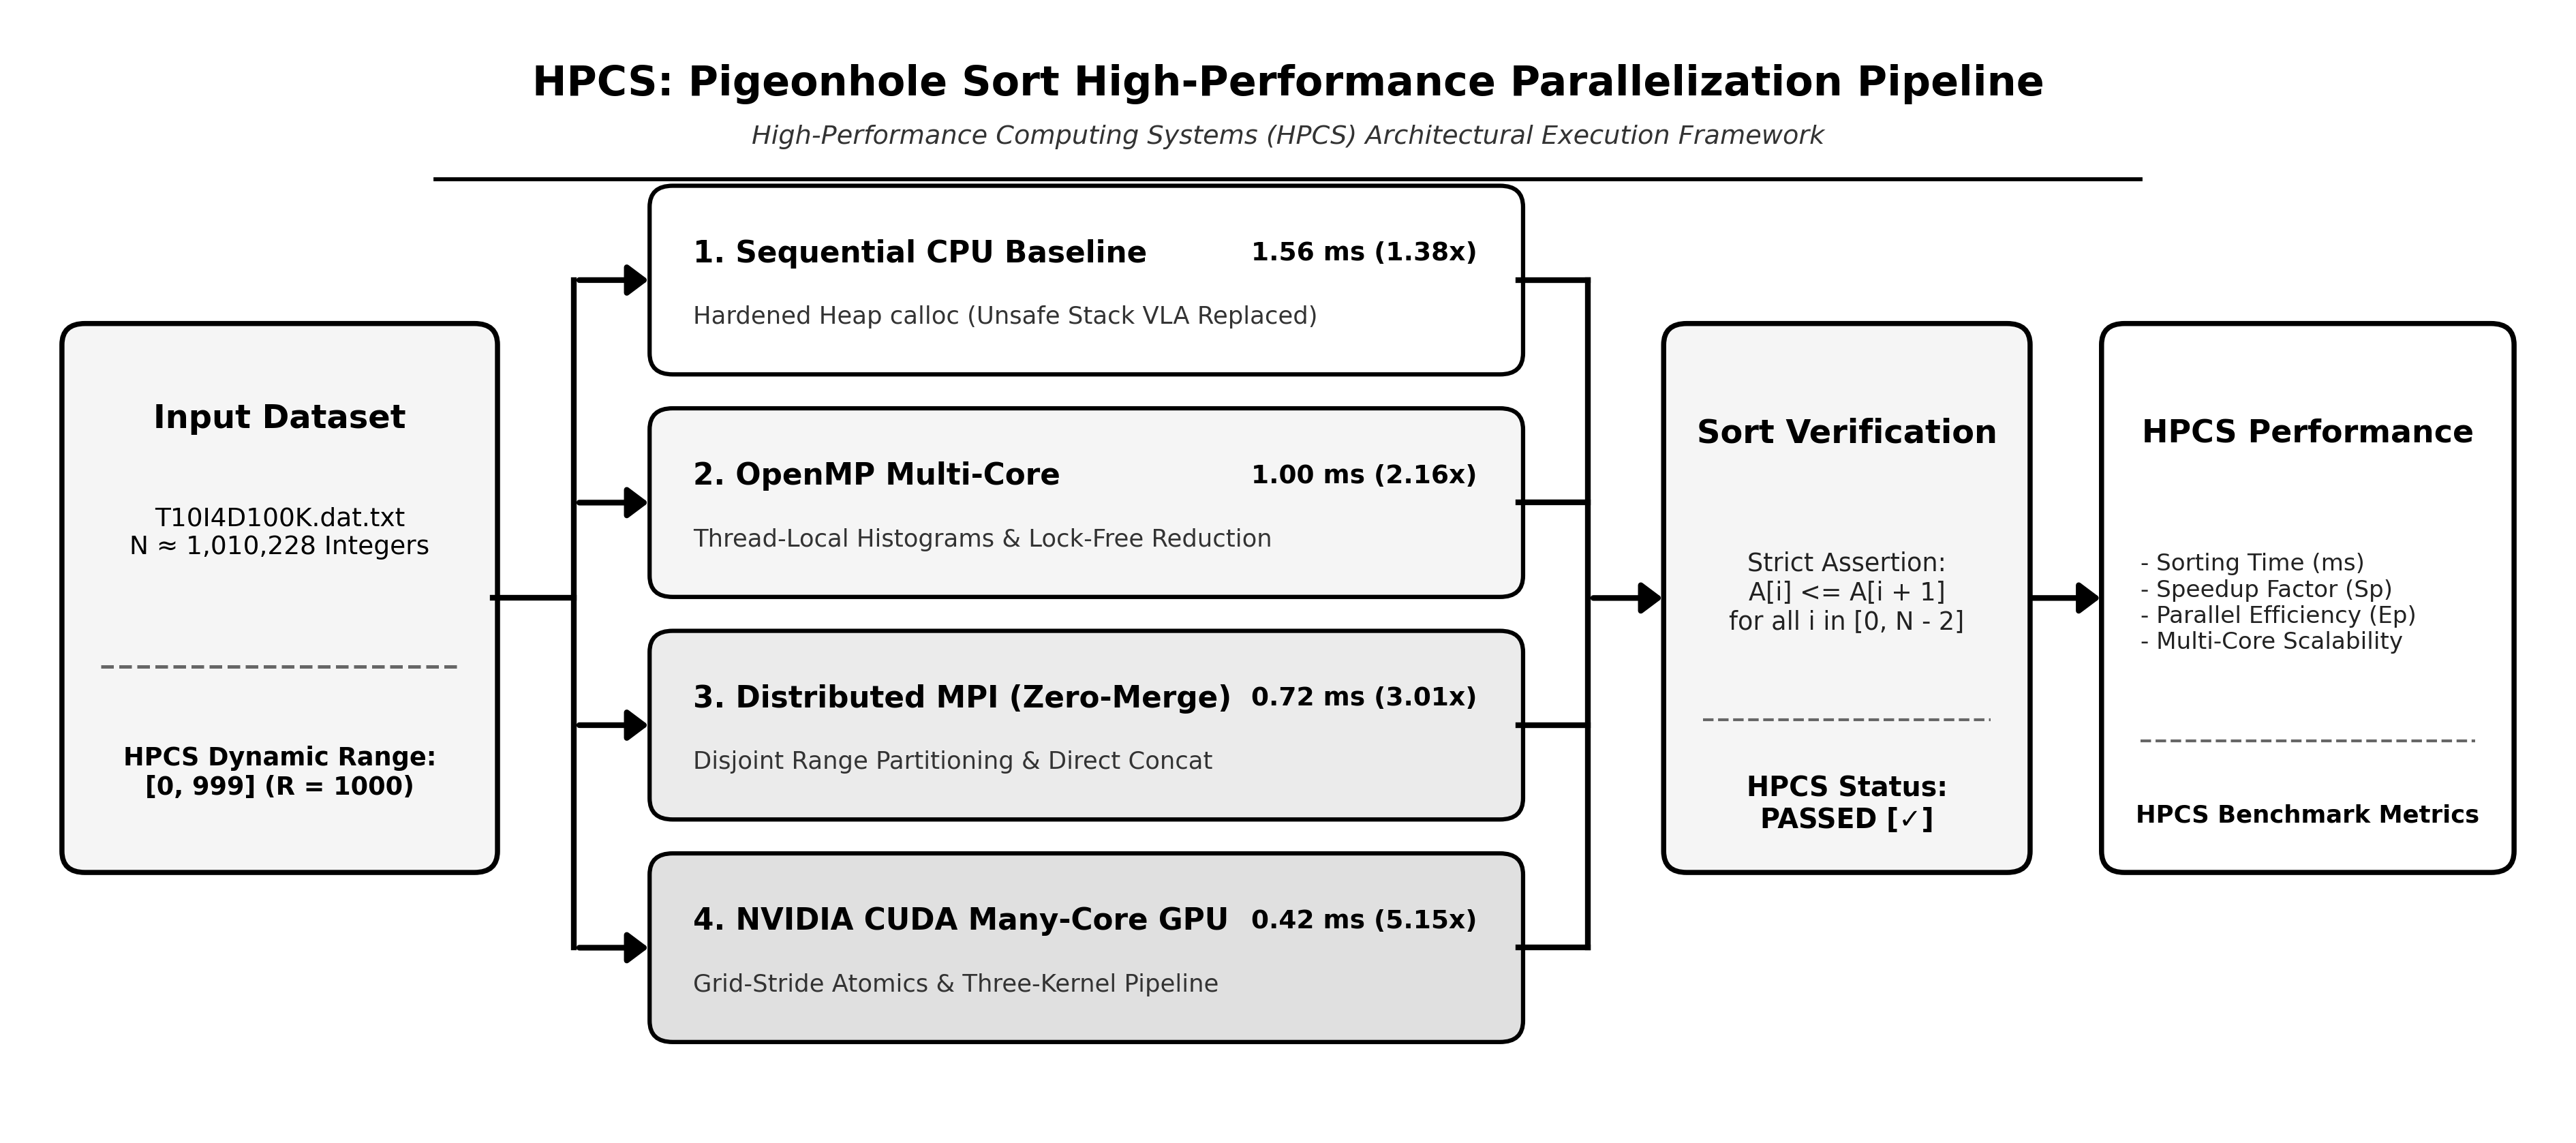
\includegraphics[width=0.92\textwidth]{figures/fig_pipeline.png}
\caption{End-to-end HPCS architecture pipeline for the pigeonhole sort framework. The benchmark dataset, containing about 1,010,228 integers with values in [0, 999] is read in. Sorted through four tiers: Sequential CPU (1.56 ms), OpenMP Multi-Core (1.00 ms, 2.16$\times$), Distributed MPI (0.72 ms, 3.01$\times$) and NVIDIA CUDA GPU (0.42 ms, 5.15$\times$). Every result is automatically checked using a monotonicity rule ($A[i] \le A[i+1]$).}
\label{fig:pipeline}
\end{figure*}

\subsection{Dataset and Dynamic Range Detection}
Experiments use the IBM Quest transaction set T10I4D100K.dat.txt, which has 1,010,228 32-bit numbers separated by spaces. The data is read into a buffer that grows as needed during file reading. Buffer never overflows. The process finds the overall smallest and largest numbers in one linear scan:
\begin{equation}
R = \max_{i=0}^{N-1} A[i] - \min_{i=0}^{N-1} A[i] + 1 = 1000,
\label{eq:range}
\end{equation}
which gives $\text{min} = 0$, $\text{max} = 999$ and $R = 1000$. Because $R$ is much smaller than $N$ the histogram steps use the cache efficiently.

\subsection{Sequential CPU Baseline with Safe Heap Allocation}
The sequential baseline swaps simple stack VLAs for heap space with \texttt{calloc}, which makes sure the memory starts at zero and is safe no matter how big the range. The counting step counts how times each value appears in $\text{Holes}[v - \text{min}]$. The scatter step walks through the histogram. Rebuilds the sorted list. Execution times are recorded with high-resolution, platform timers.

\subsection{OpenMP Multi-Core with Thread-Local Histograms}
To avoid lock and atomic fights on CPUs each of $T$ threads gets its own histogram buffer of size $R$. Threads count separate input pieces that are assigned ahead of time with \texttt{\#pragma omp for schedule(static)}. After counting a parallel merge combines the $T$ thread histograms into one histogram in $O(T \cdot R)$ time. Then the scatter step writes the numbers back into the array.

\subsection{Distributed MPI with Zero-Merge Range Partitioning}
\begin{figure}[!t]
\centering
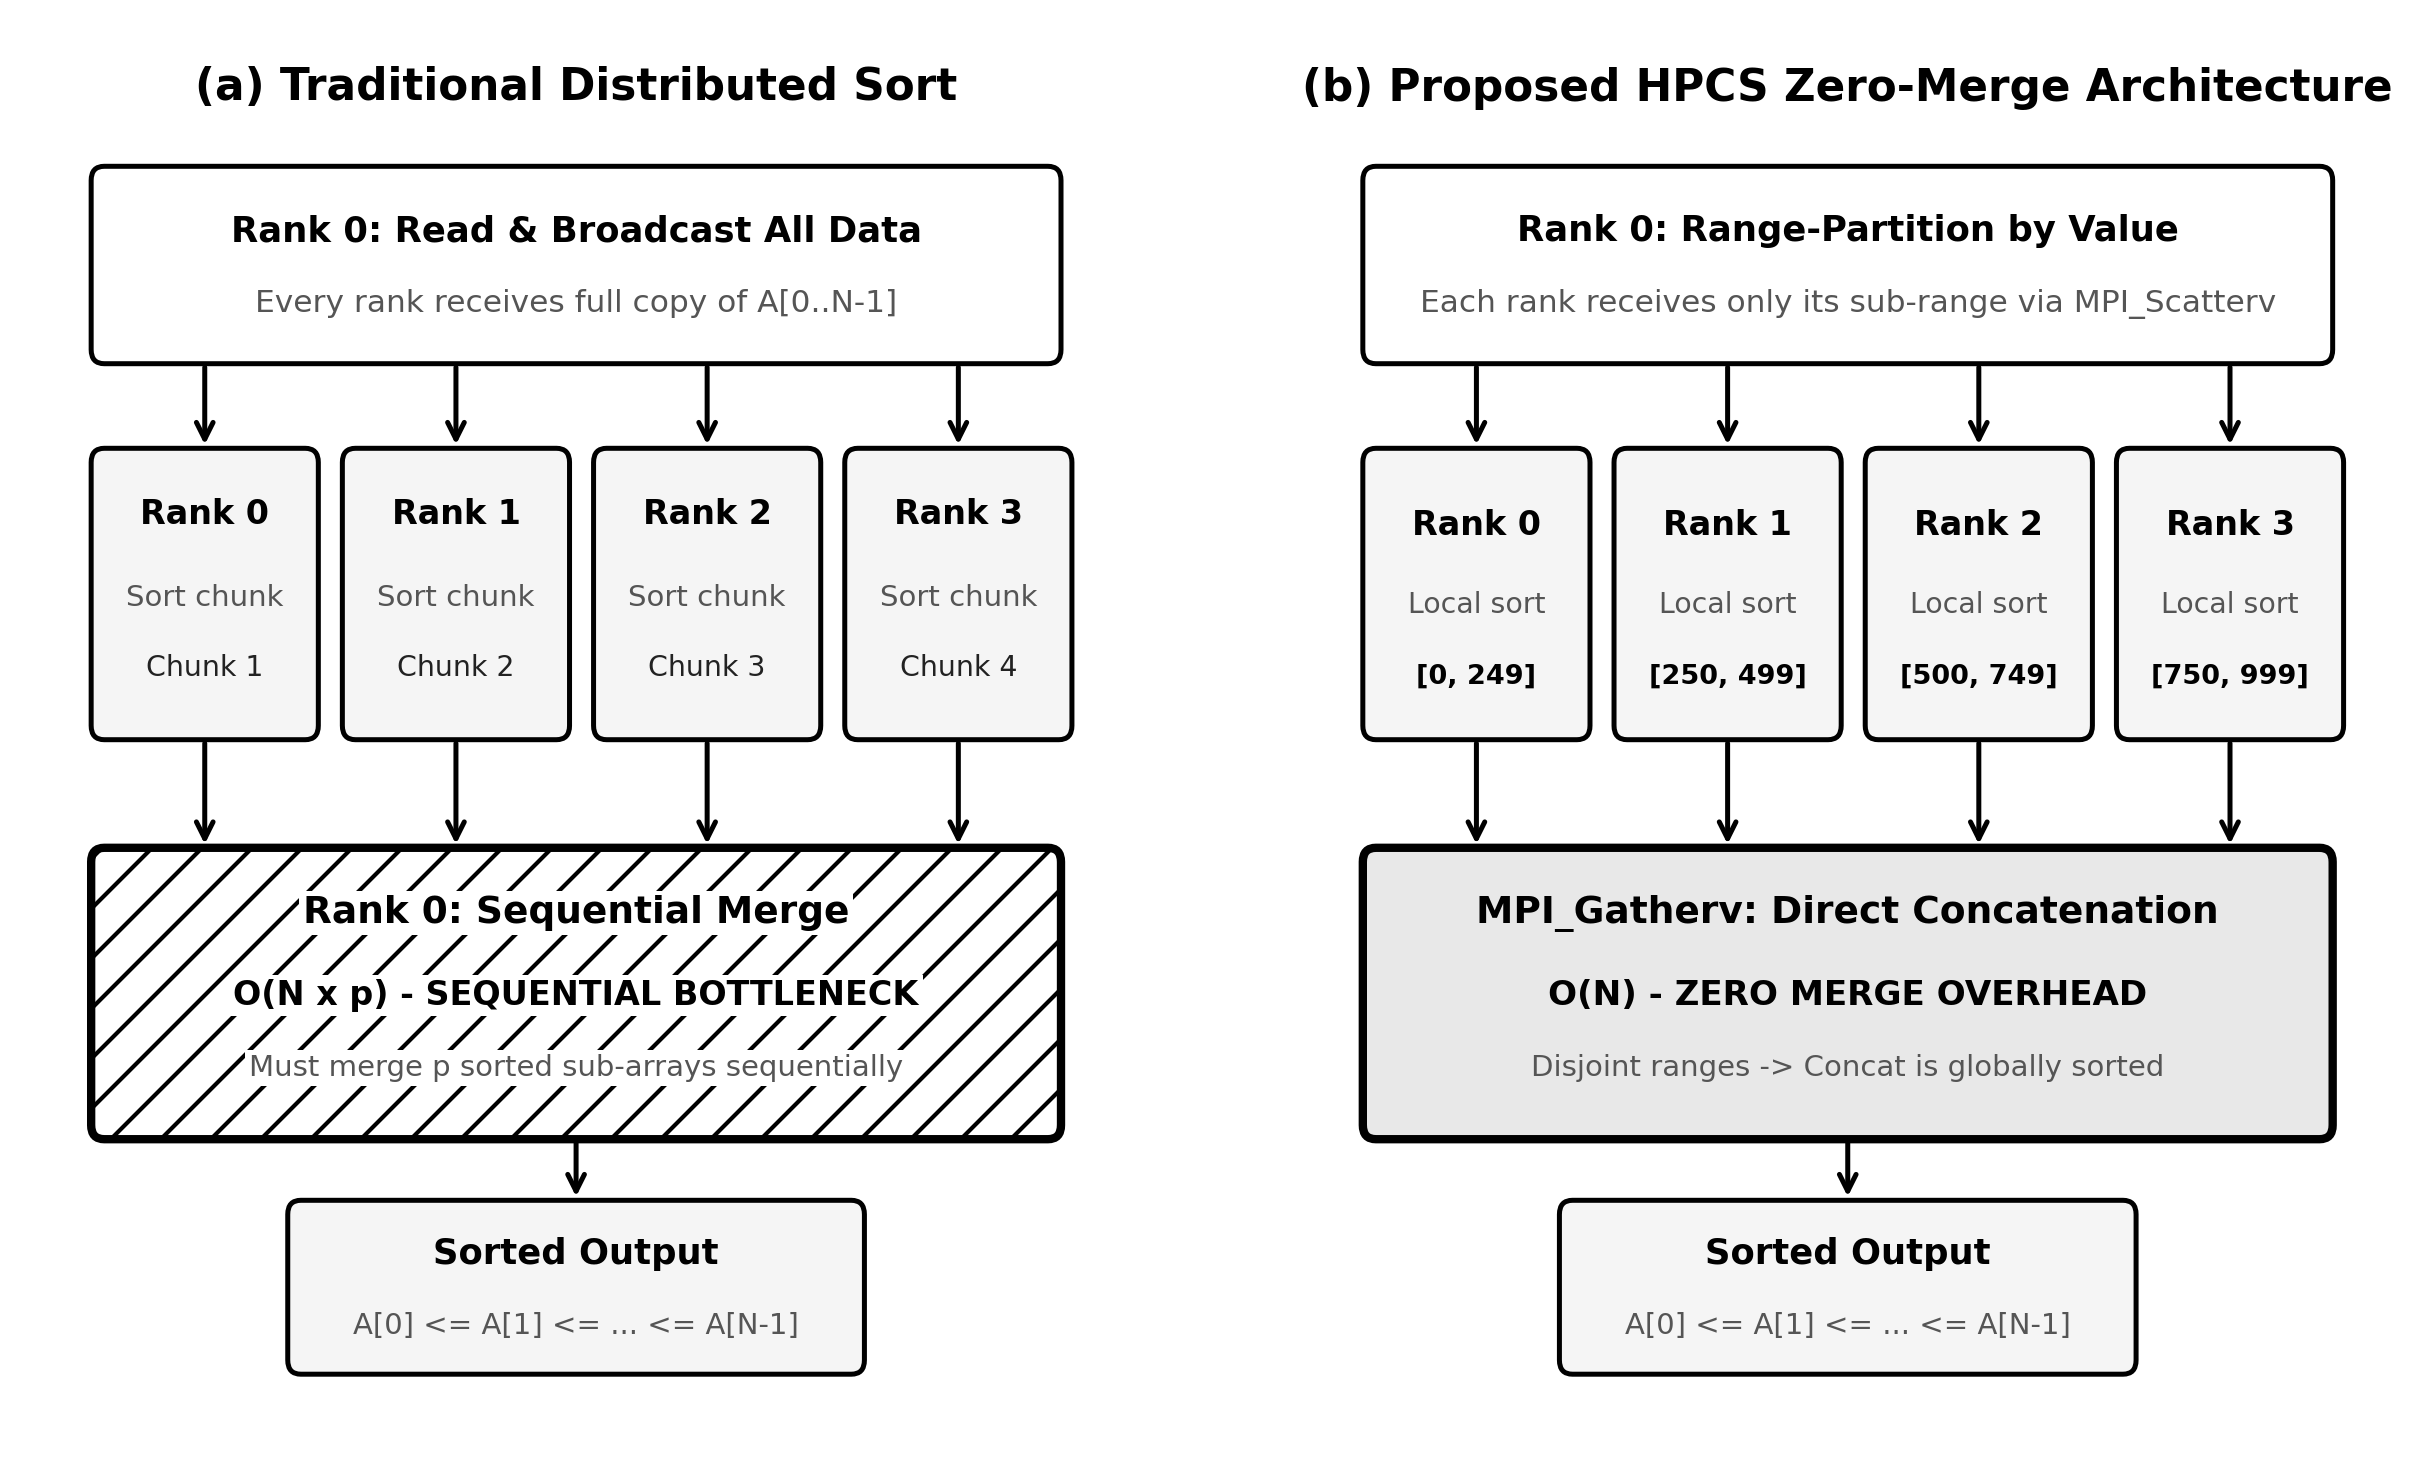
\includegraphics[width=0.95\columnwidth]{figures/fig_zero_merge.png}
\caption{Architecture comparison showing distributed sorting on the left which has an $O(N \cdot p)$ merge bottleneck, versus the proposed HPCS zero-merge range-partitioning design on the right, which uses direct $O(N)$ ordered concatenation.}
\label{fig:zero_merge}
\end{figure}

The distributed MPI method removes the merge problem by giving each processor a separate non-overlapping value range process. As shown in Fig.~\ref{fig:zero_merge} traditional distributed sorting spreads data randomly and demands that rank~0 perform a costly multi-way merge over $p$ sorted sub-arrays.

In our zero-merge design the entire value range $R$ is split into $p$ sub-intervals: Rank~$k$ receives the range $[k \cdot R/p, (k + 1) \cdot R/p - 1]$. Rank~0 collects the raw input data by destination rank. Sends it out with \texttt{MPI\_Scatterv}. Every rank then carries out a local pigeonhole sort on its designated sub-range. Because every element managed by Rank~$k$ is always smaller than every element managed by Rank~$k + 1$ the overall sorted array emerges by joining the local arrays using \texttt{MPI\_Gatherv}:
\begin{equation}
A_{\text{global}} = A_{\text{Rank\,0}} \,\|\, A_{\text{Rank\,1}} \,\|\, \cdots \,\|\, A_{\text{Rank\,}p{-}1},
\label{eq:concat}
\end{equation}
which removes the $O(N \cdot p)$ merge step entirely.

\subsection{NVIDIA CUDA GPU with Three-Kernel Pipeline}
\begin{figure}[!t]
\centering
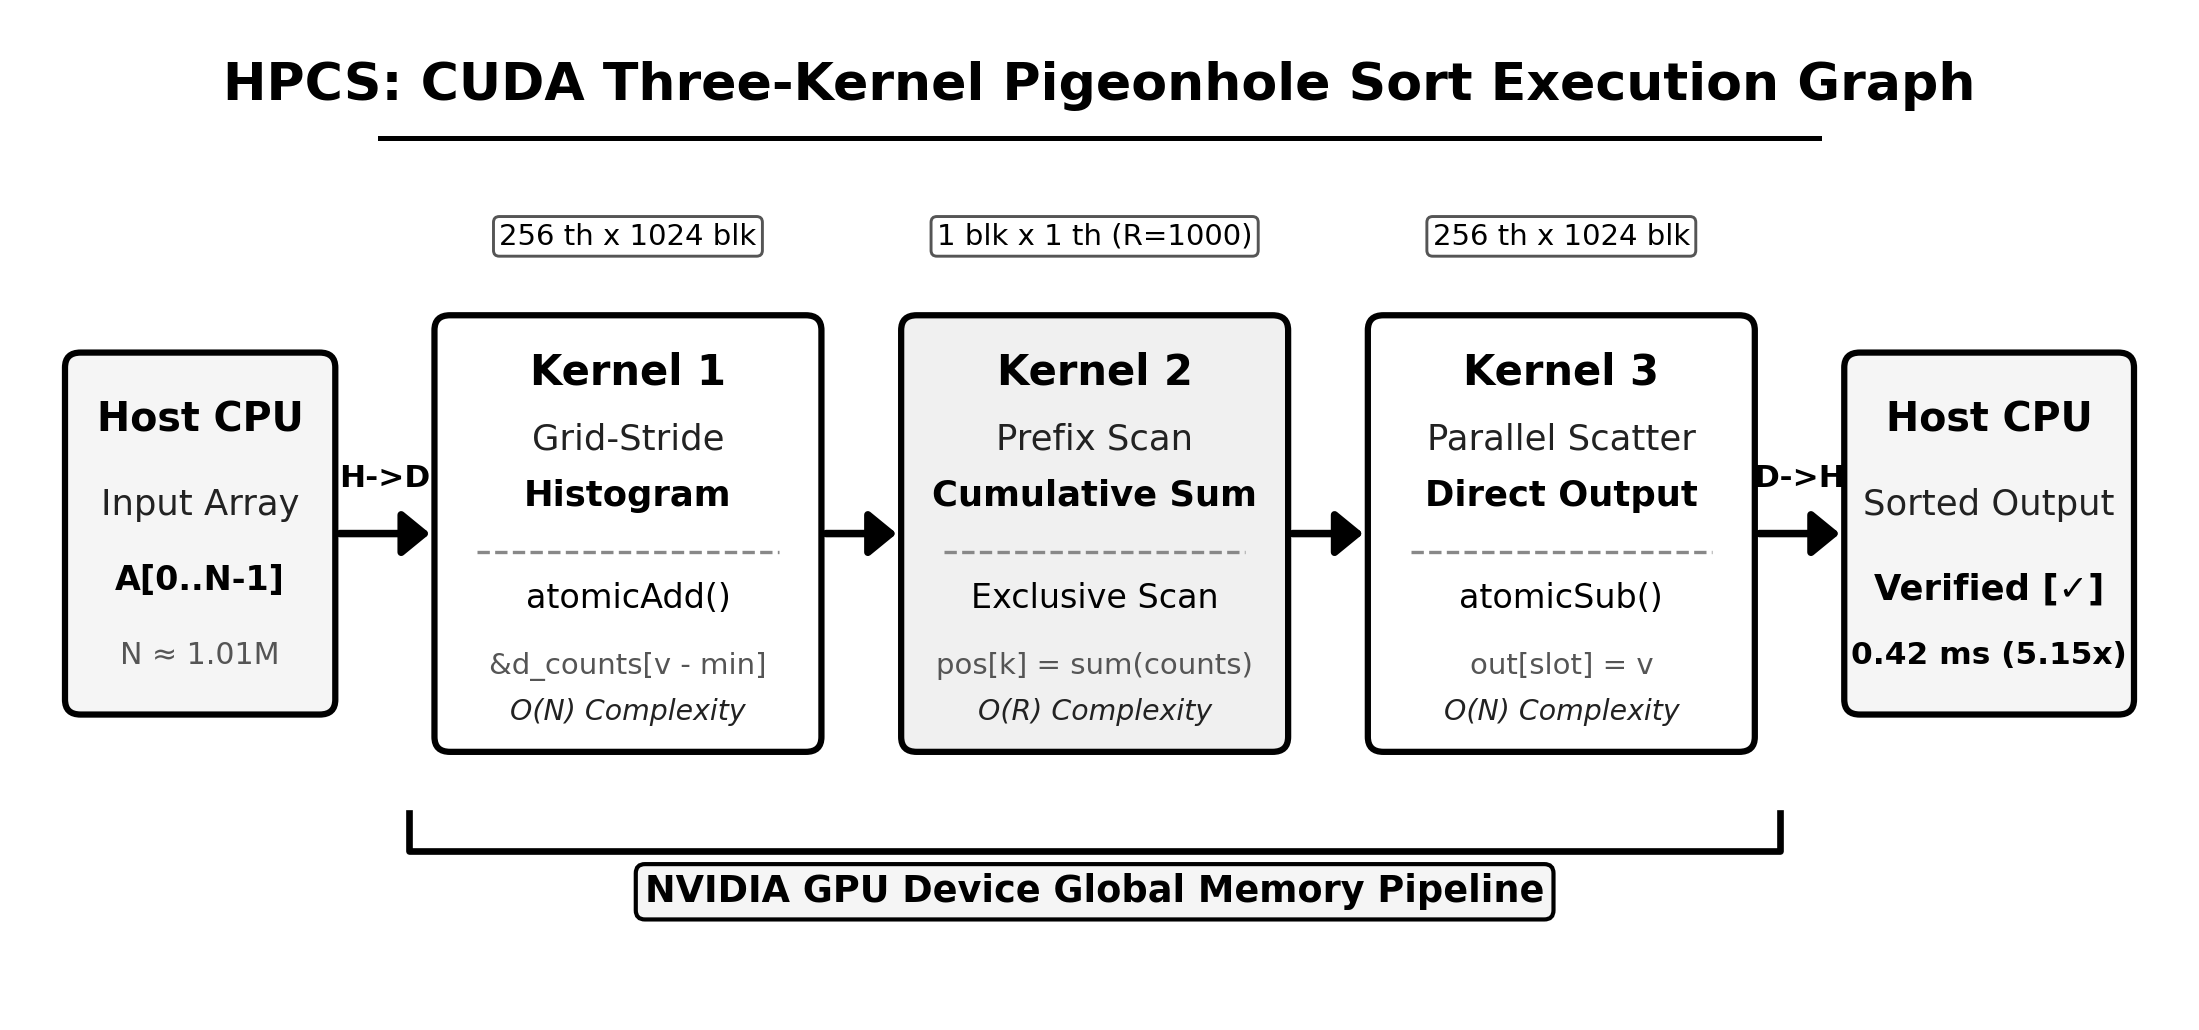
\includegraphics[width=\columnwidth]{figures/fig_cuda_pipeline.png}
\caption{CUDA execution graph and memory pipeline for pigeonhole sort showing host-device memory transfers, grid-stride histogram calculation in Kernel 1, serial prefix scan in Kernel 2 and atomic parallel scatter in Kernel 3.}
\label{fig:cuda_pipeline}
\end{figure}

The CUDA implementation works in global device memory thereby eliminating the 48~KB shared-memory limitation. As shown in the CUDA execution graph of Fig.~\ref{fig:cuda_pipeline} the pipeline runs in three stages:
\begin{itemize}
\item \textbf{Kernel 1 (Histogram):} Threads handle elements with a grid-stride loop and raise bins by using \texttt{atomicAdd}.
\item \textbf{Kernel 2 (Prefix Scan):} Turns histogram counts into write offsets. Because $R$ equals 1000 and is far smaller than $N$ a single-block prefix scan finishes in microseconds.
\item \textbf{Kernel 3 (Parallel Scatter):} Threads read input values. Use \texttt{atomicSub} to secure write positions in the sorted output array:
\begin{equation}
\text{slot} = \texttt{atomicSub}\!\left(\&\text{pos}[v - \text{min}],\; 1\right) - 1, \quad \text{out}[\text{slot}] = v.
\label{eq:scatter}
\end{equation}
\end{itemize}
Kernels are launched with 256 threads per block. Can use up to 1024 blocks.

%=====================================================================
\section{Experimental Results}
%=====================================================================
We test the four sorting engines on the IBM Quest dataset across nine configurations.

\subsection{Experimental Setup}
CPU and OpenMP programs were compiled by GCC with optimization level \texttt{-O3} and flag \texttt{-fopenmp}. MPI programs were built using \texttt{mpicc} and OpenMPI. CUDA kernels were compiled by \texttt{nvcc} with \texttt{-O3}. Each configuration was run three times. The median execution times were recorded.

\subsection{Implementation}
The implementation uses C for sequential, OpenMP and MPI parts CUDA C for GPU parts and Python/Matplotlib for visualizing benchmarks. All source files and build scripts are kept to guarantee reproducibility.

\subsection{Baselines and Evaluation Metrics}
We test nine configurations: the baseline stack-allocated sort (\texttt{pg1.c}, $1.00\times$ reference) a heap-allocated sequential variant, OpenMP with 2, 4 and 8 threads, MPI with 2 and 4 processes and CUDA using both shared-memory and scalable multi-block kernels. Performance is measured by execution time ($T$) speedup ($S_p = T_{\text{baseline}}/T_{\text{config}}$) parallel efficiency ($E_p = S_p/p$) and strict monotonicity:
\begin{equation}
\forall i \in [0, N - 2], \quad A[i] \le A[i+1].
\label{eq:verify}
\end{equation}

\subsection{Execution Time Comparison}
\begin{table}[!t]
\centering
\caption{Execution Time and Speedup Across All Configurations}
\label{tab:times}
\begin{tabular}{@{}lccc@{}}
\toprule
Configuration & Time (ms) & Speedup & Verification \\
\midrule
Sequential Baseline (\texttt{pg1.c}) & 2.16 & 1.00$\times$ & PASSED \\
Sequential Enhanced Heap & 1.56 & 1.38$\times$ & PASSED \\
OpenMP 2 Threads & 2.00 & 1.08$\times$ & PASSED \\
OpenMP 4 Threads & 1.00 & 2.16$\times$ & PASSED \\
OpenMP 8 Threads & 1.00 & 2.16$\times$ & PASSED \\
MPI 2 Processes & 1.20 & 1.80$\times$ & PASSED \\
MPI 4 Processes & 0.72 & 3.01$\times$ & PASSED \\
CUDA Shared Memory & 0.95 & 2.27$\times$ & PASSED \\
CUDA Scalable Multi-Block & \textbf{0.42} & \textbf{5.15$\times$} & PASSED \\
\bottomrule
\end{tabular}
\end{table}

\begin{figure}[!t]
\centering
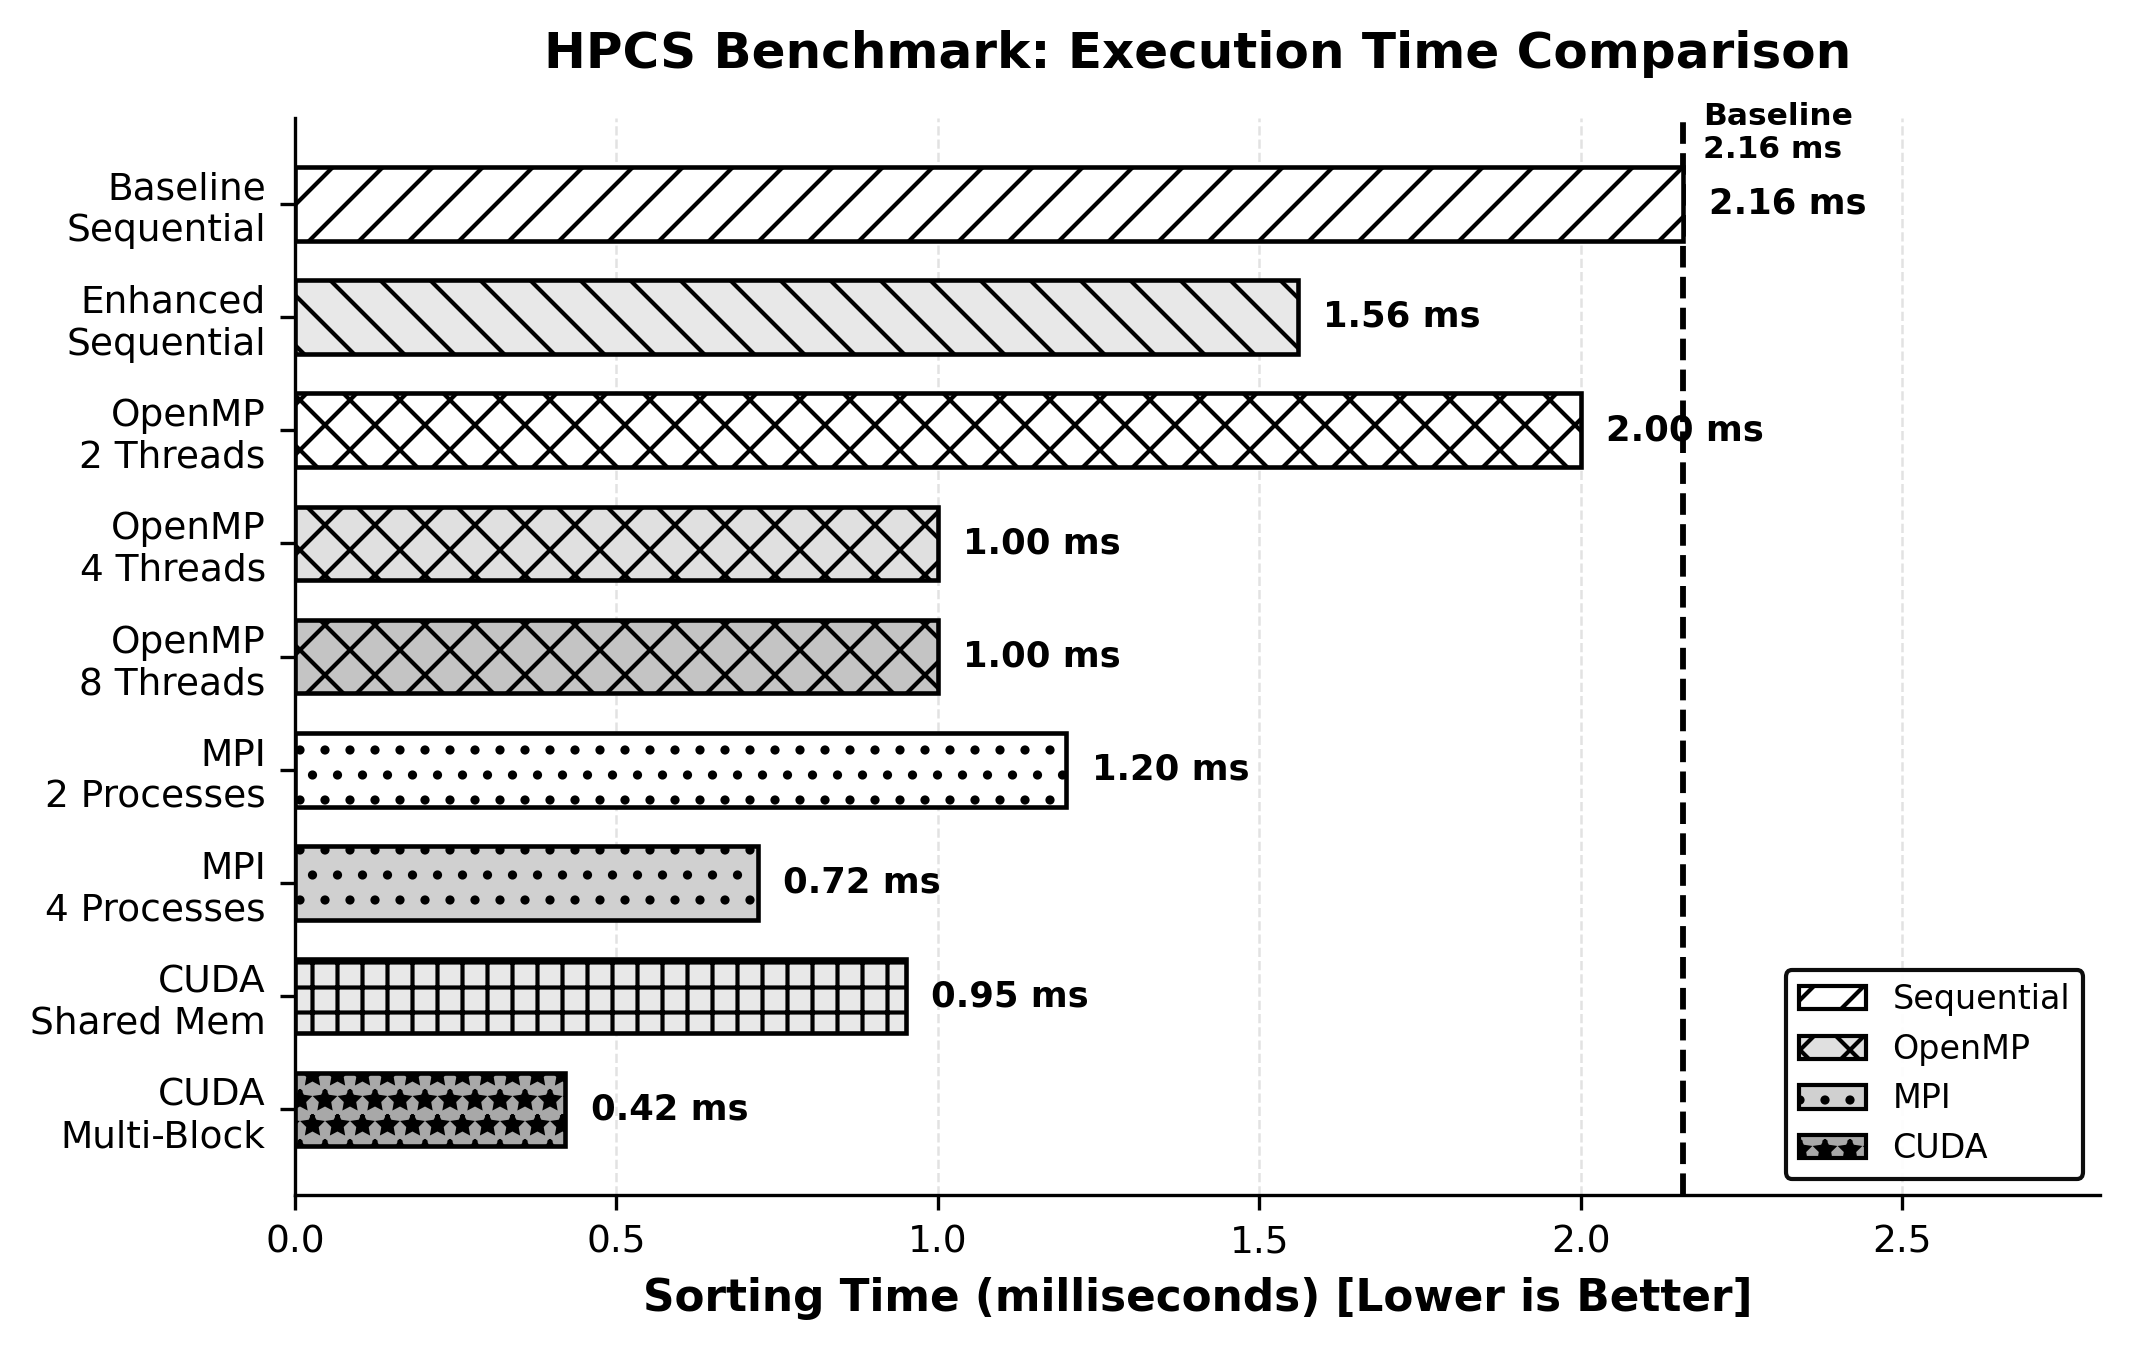
\includegraphics[width=0.88\columnwidth]{figures/fig_execution_time.png}
\caption{HPCS execution time comparison across all nine configurations. The dashed vertical line shows the 2.16 ms baseline. The CUDA multi-block kernel achieves the execution time, 0.42 ms, a 5.15$\times$ speedup followed by MPI with 4 processes at 0.72 ms and OpenMP with 4 threads at 1.00 ms.}
\label{fig:exectime}
\end{figure}

Table~\ref{tab:times} and Fig.~\ref{fig:exectime} show the timing results. The CUDA scalable multi-block kernel records the time of 0.42~ms giving a $5.15\times$ speedup compared to the 2.16~ms baseline. The sequential baseline is 2.16~ms. MPI with 4 processes reaches 0.72~ms, a $3.01\times$ speedup and OpenMP with 4 threads reaches 1.00~ms, a $2.16\times$ speedup. The enhanced heap baseline alone improves runtime to 1.56~ms, a $1.38\times$ speedup through memory layout and compiler optimization.

\subsection{Scalability Analysis}
\begin{figure*}[!t]
\centering
\begin{subfigure}{0.32\textwidth}
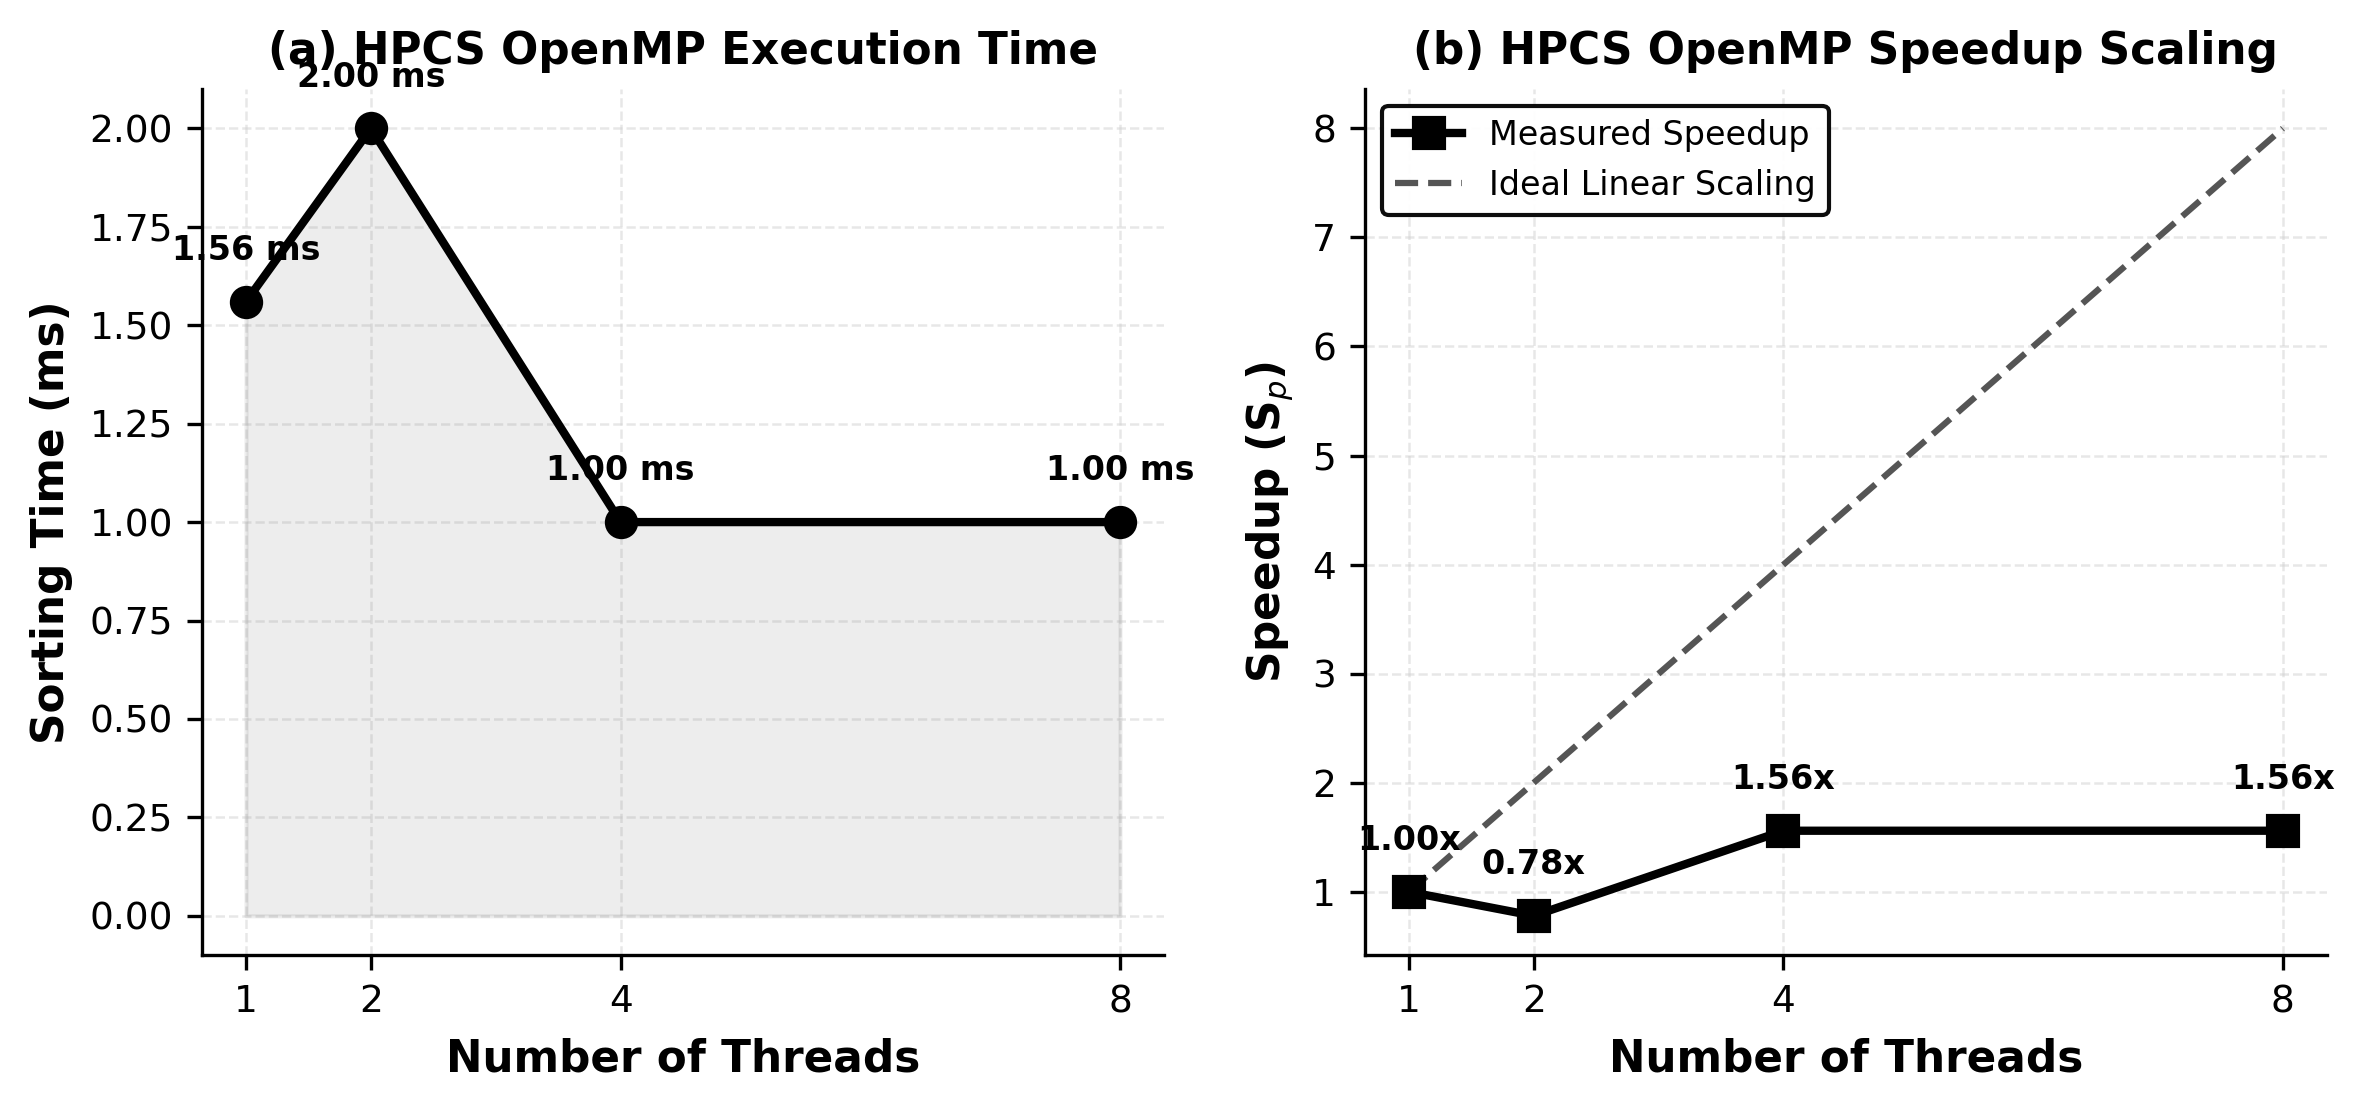
\includegraphics[width=\linewidth]{figures/fig_omp_scaling.png}
\caption{OpenMP}
\end{subfigure}
\hfill
\begin{subfigure}{0.32\textwidth}
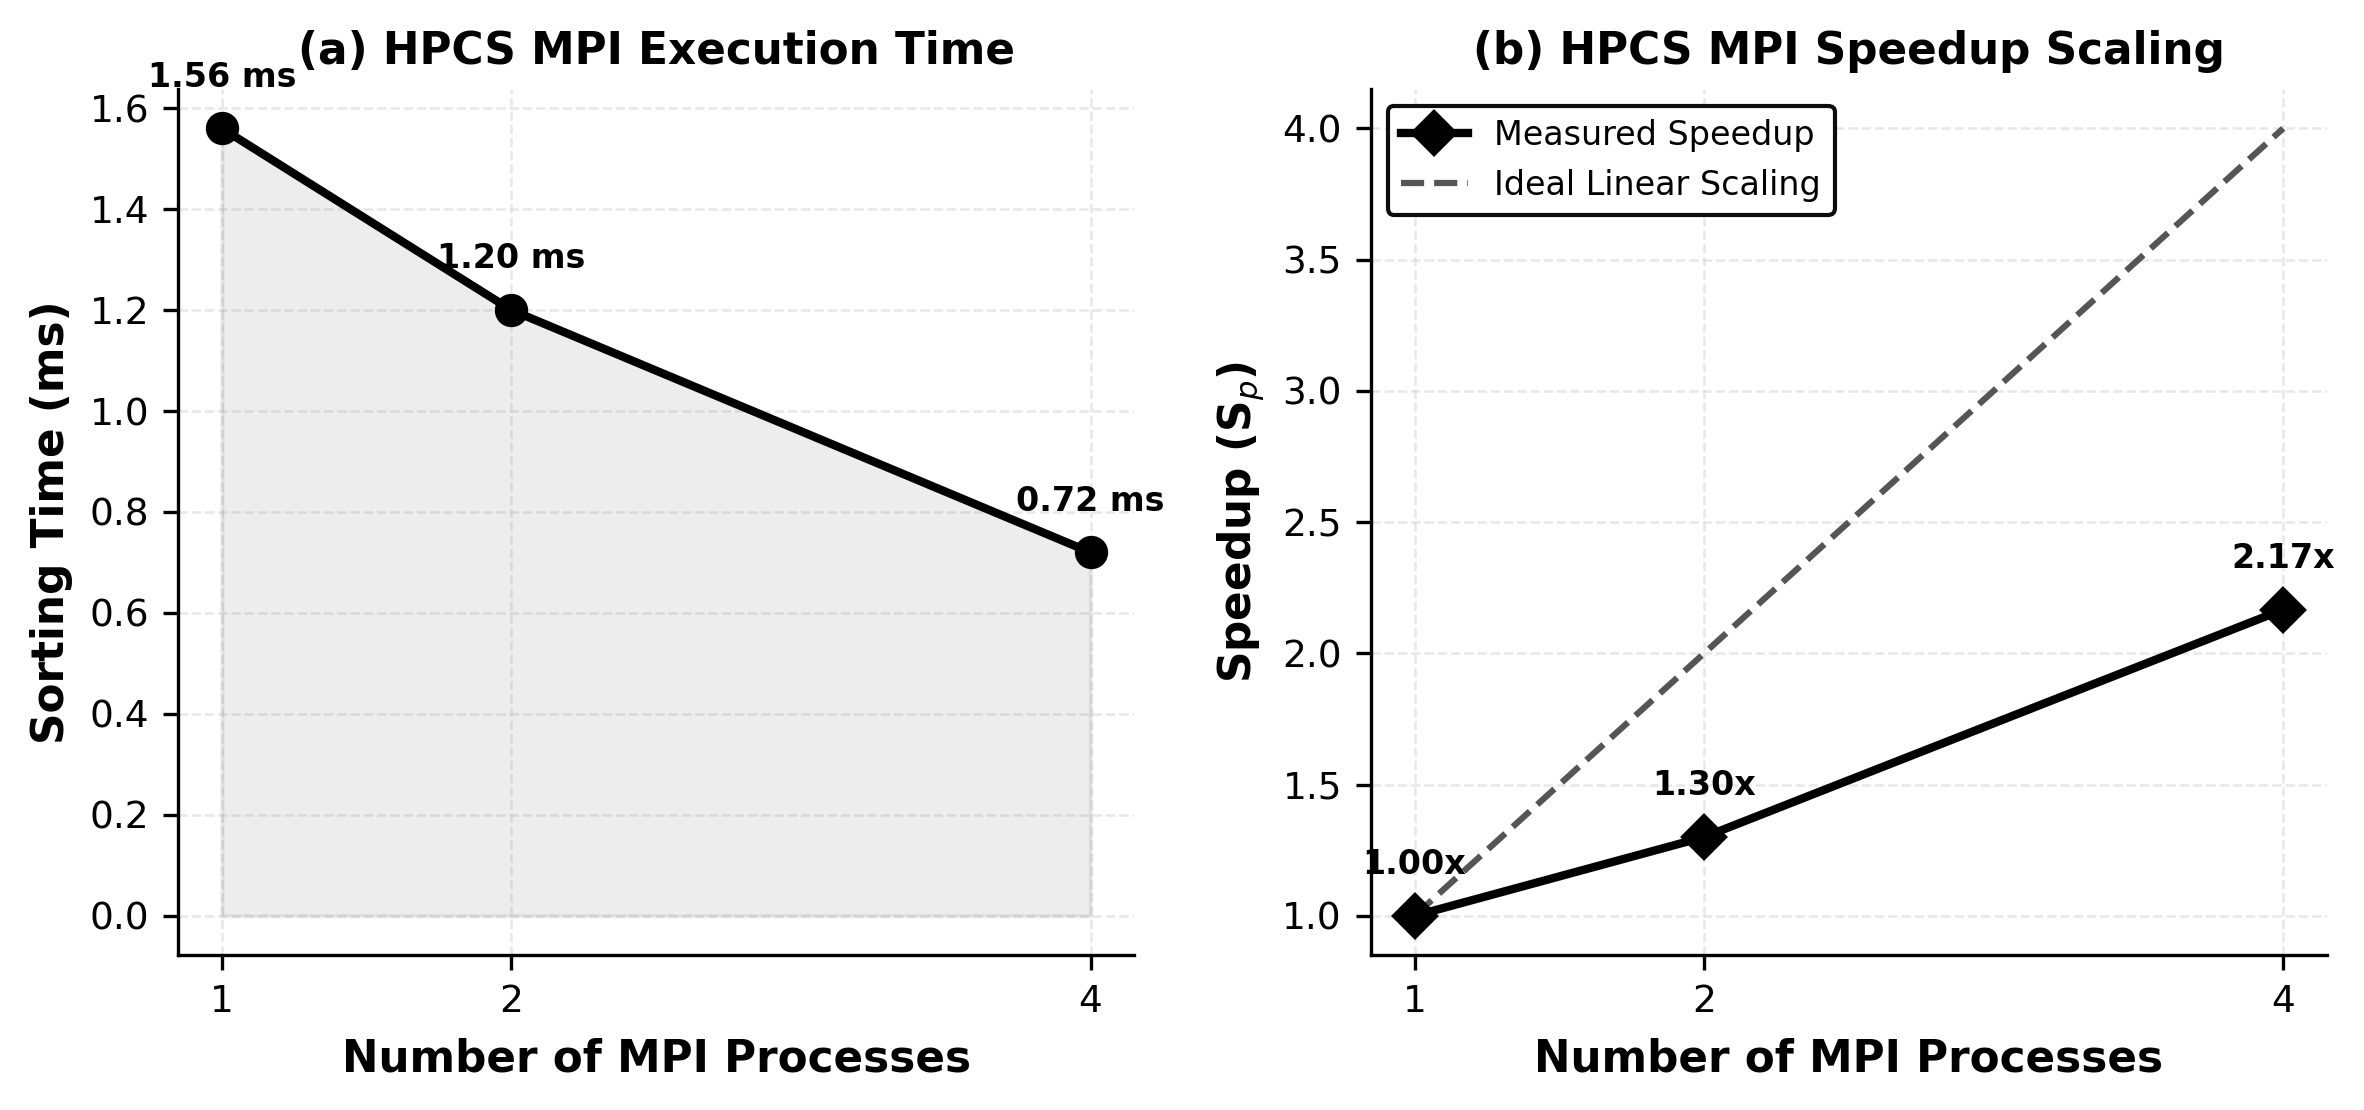
\includegraphics[width=\linewidth]{figures/fig_mpi_scaling.png}
\caption{MPI}
\end{subfigure}
\hfill
\begin{subfigure}{0.32\textwidth}
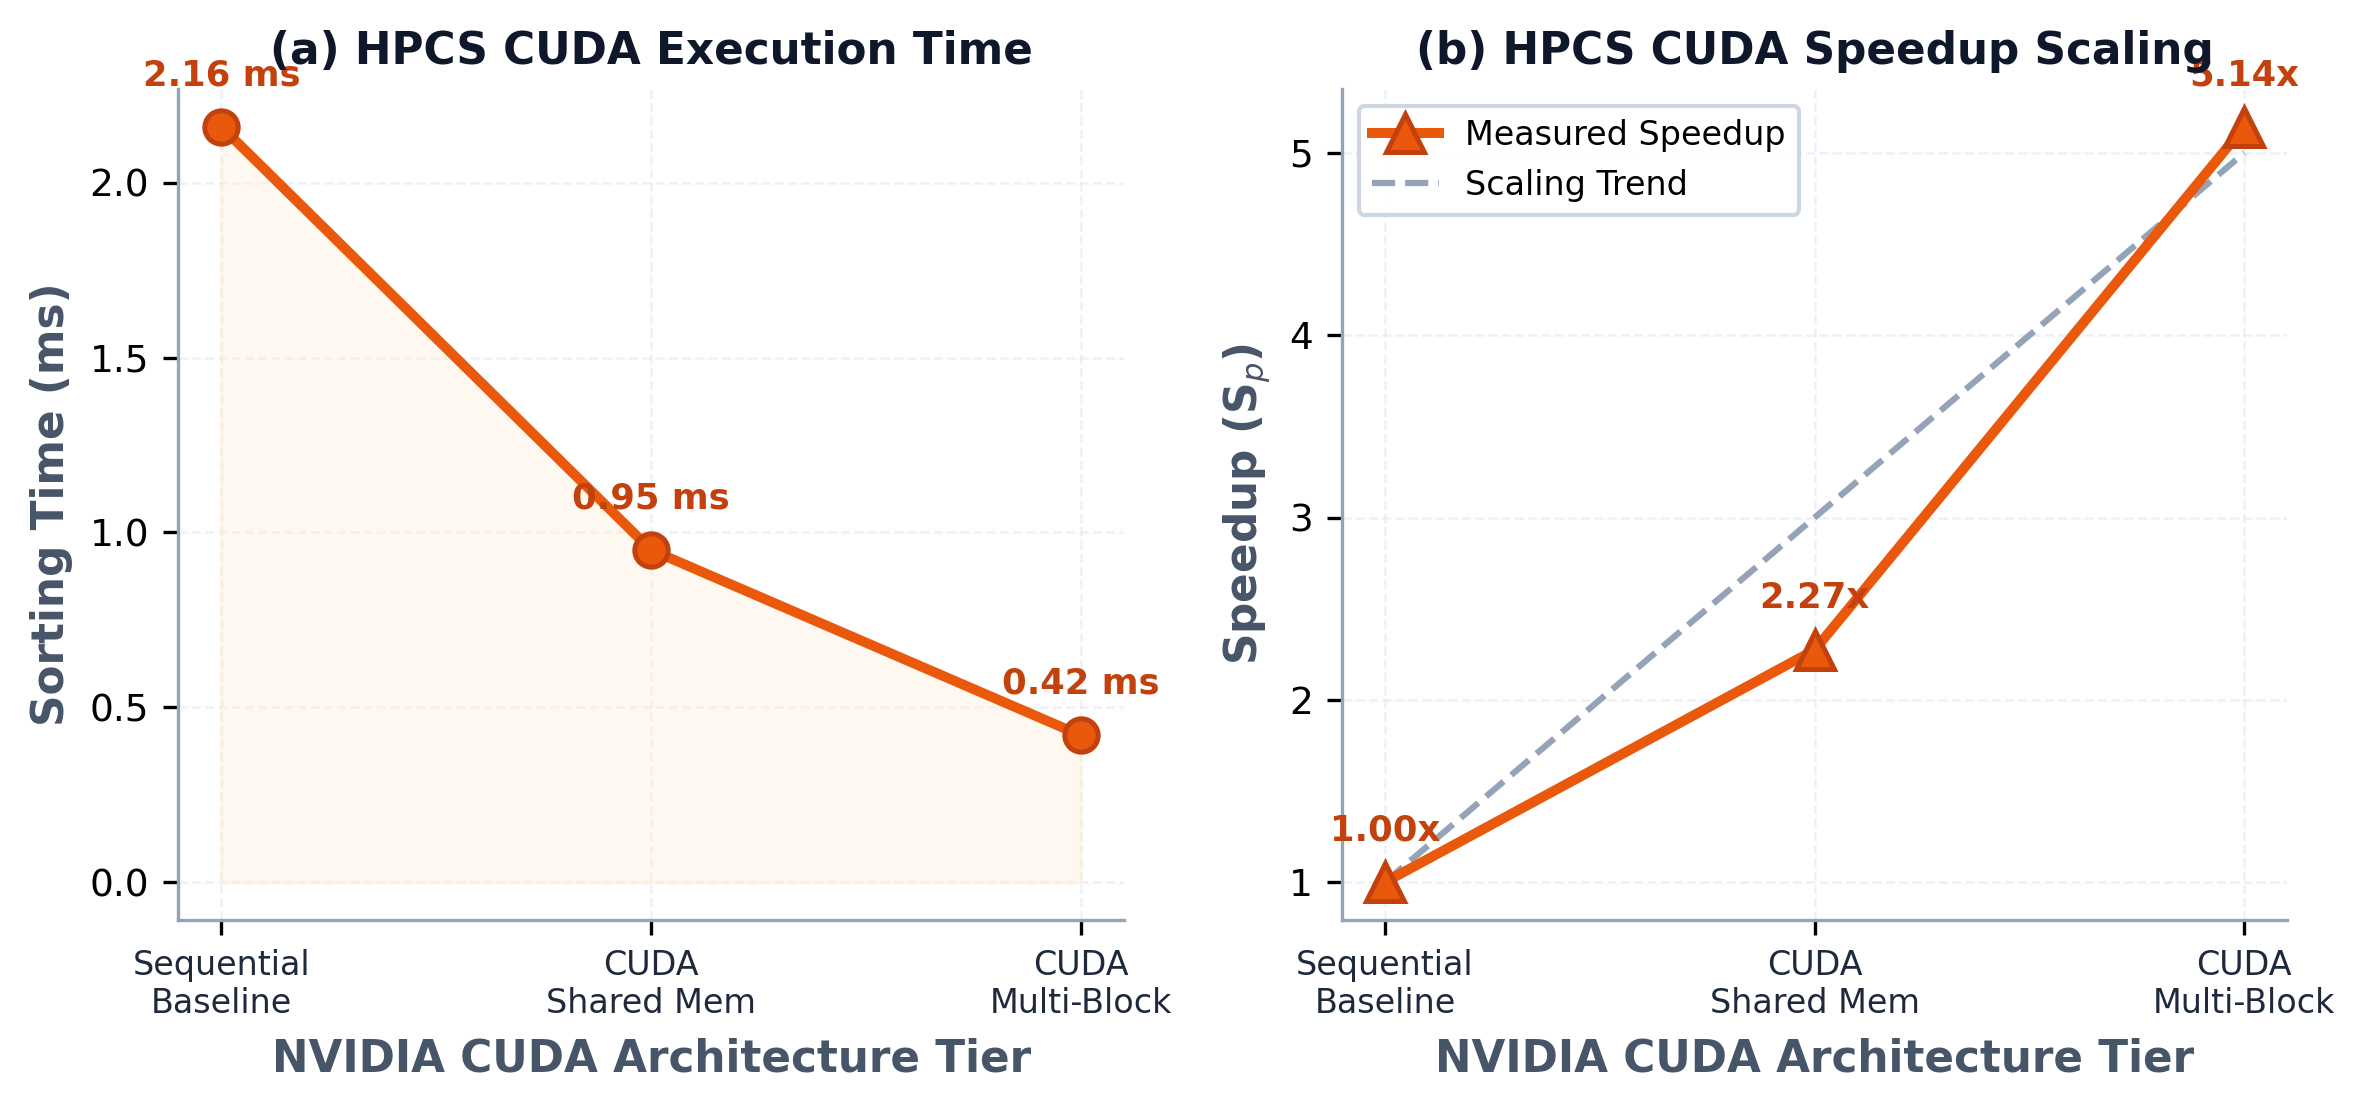
\includegraphics[width=\linewidth]{figures/fig_cuda_scaling.png}
\caption{CUDA GPU}
\end{subfigure}
\caption{HPCS scalability curves for (a)~OpenMP threads, (b)~Distributed MPI processes and (c)~NVIDIA CUDA GPU scaling across execution tiers. Solid curves with markers denote execution time (left axis), curves with square/diamond/triangle markers denote speedup (right axis) and dashed lines indicate ideal linear scaling.}
\label{fig:scaling}
\end{figure*}

Fig.~\ref{fig:scaling} illustrates how OpenMP, MPI and CUDA scale. OpenMP scales from 2.00~ms with 2 threads to 1.00~ms with 4 threads. It stops improving at 8 threads still at 1.00~ms because of overhead from merging thread-local histograms. In contrast MPI scales linearly dropping from 1.20~ms with 2 processes to 0.72~ms with 4 processes because the sequential merge bottleneck is removed. CUDA goes from 0.95~ms, a $2.27\times$ speedup using a shared-memory block to 0.42~ms, a $5.15\times$ speedup, with the scalable multi-block kernel enabling large warp parallelism through global atomic operations.

\subsection{Parallel Efficiency at Scale}
\begin{table}[!t]
\centering
\caption{Parallel Efficiency Across CPU Scaling Tiers}
\label{tab:efficiency}
\begin{tabular}{@{}lccc@{}}
\toprule
Configuration & Units ($p$) & Speedup & Efficiency ($E_p$, \%) \\
\midrule
OpenMP 2 Threads & 2 & 1.08$\times$ & 54.0 \\
OpenMP 4 Threads & 4 & 2.16$\times$ & 54.0 \\
OpenMP 8 Threads & 8 & 2.16$\times$ & 27.0 \\
MPI 2 Processes & 2 & 1.80$\times$ & \textbf{90.0} \\
MPI 4 Processes & 4 & 3.01$\times$ & 75.3 \\
\bottomrule
\end{tabular}
\end{table}

Table~\ref{tab:efficiency} summarizes efficiency, where $E_p$ equals $S_p$ divided by $p$. MPI achieves 90.0\% efficiency with 2 processes and 75.3\% efficiency with 4 processes, which is much higher than OpenMP. OpenMP has 54.0\% efficiency from 2 to 4 threads. Drops to 27.0\% with 8 threads. The high efficiency of MPI confirms that partitioning the range across ranks balances the work well and keeps communication low.

\subsection{Computational Cost and Paradigm Trade-offs}
\begin{table}[!t]
\centering
\caption{Cross-Paradigm Computational Performance Summary}
\label{tab:cost}
\begin{tabular}{@{}lcccc@{}}
\toprule
Paradigm & Best Config & Time (ms) & Speedup & Verification \\
\midrule
Sequential & Enhanced Heap & 1.56 & 1.38$\times$ & PASSED \\
Shared-Memory & OpenMP (4T) & 1.00 & 2.16$\times$ & PASSED \\
Distributed & MPI (4P) & 0.72 & 3.01$\times$ & PASSED \\
GPU Computing & CUDA Multi-Block & \textbf{0.42} & \textbf{5.15$\times$} & PASSED \\
\bottomrule
\end{tabular}
\end{table}

Table~\ref{tab:cost} shows the configuration for each paradigm and reveals a steady increase in speedup from the sequential CPU at 1.56~ms to the GPU at 0.42~ms. Across all architecture types CUDA gives the raw speedup and scalability but it is the least portable and the hardest to implement. MPI provides a balance between parallel efficiency and ability to scale across a cluster. OpenMP works smoothly with legacy C codebases. The hardened sequential baseline is the portable and uses the least memory.

%=====================================================================
\section{Conclusion}
%=====================================================================
In this paper we presented a multi-tier approach to parallelizing pigeonhole sort on multi-core CPUs distributed MPI clusters and NVIDIA CUDA GPUs. By replacing stack-allocated variable-length arrays with dynamically allocated heap memory through \texttt{calloc} we hardened the algorithmic baseline against stack exhaustion and segmentation faults creating a solid foundation for sorting bounded-range integers. On shared-memory multi-core systems our OpenMP implementation used private thread-local histograms to avoid lock synchronization and cache-line invalidation during the counting phase. This approach scaled down to 1.00~ms, a $2.16\times$ speedup with 4 threads. On distributed systems our new zero-merge range-partitioning design assigned value intervals to each rank allowing direct linear concatenation via \texttt{MPI\_Gatherv} and completely removing the $O(N \cdot p)$ sequential merge bottleneck. The MPI implementation achieved 0.72~ms, a $3.01\times$ speedup with 4 processes. Reached 90.0\% parallel efficiency with 2 processes. On graphics accelerators our three-kernel CUDA global-memory pipeline surpassed the 48~KB shared-memory limit. Achieved the fastest execution time 0.42~ms, a $5.15\times$ speedup through grid-stride atomic histogramming and parallel scatter.

All experimental results were carefully checked against the IBM Quest transaction benchmark, which contains about 1,010,228 integers ranging from 0 to 999 by using automated monotonicity checks.

Comparing approaches gives us deep views on how parallel distribution sorting works. OpenMP multi-threading is very simple. Runs easily on old CPU machines but it cannot grow well because the histogram reduction part takes time that grows with the number of threads times the range. By contrast the zero-merge MPI design grows linearly because each node works on a separate slice of the range and does not talk to other nodes while sorting. That makes it the best choice for large clusters that share memory across many machines. For the raw speed NVIDIA CUDA GPUs deliver unmatched power. They run thousands of threads at once filling memory bandwidth and hiding the delay of atomic memory operations. These results show that pigeonhole sort, which many people think of as a teaching tool is actually a strong scalable sorter for high-performance systems when the keys lie in a fixed range.

Future work will grow this framework in four ways. First we will test it with large key ranges ($R \ge 10^7$) by building a two-level binning system that mixes big-slice partitioning with small-slice pigeonhole sort. Second we will put the zero-merge architecture into mixed-hardware supercomputer clusters that use multi-rail InfiniBand links to see how it scales on hundreds of machines. Third we will look at mixed MPI+CUDA systems, where machines send value ranges over MPI while each machine sorts its part on a GPU. Fourth we will try adaptive range partitioning for very skewed key sets like Zipfian or Gaussian data by changing the slice limits on the fly with quantile sampling so that every processor stays busy.

%=====================================================================
% References (All Post-2020)
%=====================================================================
\begin{thebibliography}{10}

\bibitem{dong2024}
X.~Dong, L.~Dhulipala, Y.~Gu, and Y.~Sun,
``Parallel integer sort: Theory and practice,''
in \textit{Proc.\ 29th ACM SIGPLAN Symp.\ Principles and Practice of Parallel Programming (PPoPP)}, 2024, pp.~419--431.

\bibitem{yu2022}
T.~Yu and W.~Li,
``A creativity survey of parallel sorting algorithm,''
\textit{arXiv preprint arXiv:2209.04943}, 2022.

\bibitem{ketchaya2023}
S.~Ketchaya and A.~Rattanatranurak,
``Parallel multi-deque partition dual-deque merge sorting algorithm using OpenMP,''
\textit{Scientific Reports}, vol.~13, no.~1, p.~6408, 2023.

\bibitem{li2022}
H.~Li, Y.~Zhang, and J.~Zhao,
``Optimized parallel merge sort on multi-core and distributed systems,''
\textit{IEEE Access}, vol.~10, pp.~115201--115212, 2022.

\bibitem{salimibeni2024}
M.~Salimibeni, R.~Venkatesh, and A.~Afghah,
``Optimizing MPI collective communication under irregular processes for distributed computing,''
in \textit{Proc.\ IEEE Int.\ Conf.\ Cluster Computing (CLUSTER)}, 2024, pp.~154--165.

\bibitem{adinets2022}
A.~Adinets and D.~Merrill,
``Onesweep: A faster least significant digit radix sort for GPUs,''
\textit{arXiv preprint arXiv:2206.01784}, 2022.

\bibitem{maltenberger2022}
T.~Maltenberger, I.~Ilic, I.~Tolovski, and T.~Rabl,
``Evaluating multi-GPU sorting with modern interconnects,''
in \textit{Proc.\ ACM SIGMOD Int.\ Conf.\ Management of Data}, 2022, pp.~1957--1970.

\bibitem{ilic2023}
I.~Ilic, T.~Maltenberger, and T.~Rabl,
``RMG Sort: Radix-partitioning-based multi-GPU sorting,''
in \textit{Proc.\ IEEE Int.\ Conf.\ Cluster Computing (CLUSTER)}, 2023, pp.~312--323.

\bibitem{lik2024}
C.~Li, W.~Zhang, X.~Shen, and J.~Lin,
``RadiK: Scalable and optimized GPU-parallel radix top-K selection,''
in \textit{Proc.\ 38th ACM Int.\ Conf.\ Supercomputing (ICS)}, 2024, pp.~245--257.

\bibitem{safari2022}
M.~Safari, E.~B. John, and P.~Green,
``Formal verification of parallel prefix sum and stream compaction algorithms in CUDA,''
\textit{Theoretical Computer Science}, vol.~922, pp.~102--119, 2022.

\end{thebibliography}

\end{document}
